\chapter{系统案例测试分析}

本节旨在展示系统在自然语言驱动的交通场景生成任务中的实际运行效果。通过选取多个具有代表性的输入示例,分别涵盖了不同类型的交通语义指令,如静态车道场景、红绿灯交叉口、雨天行车、复杂车辆交汇等,全面体现系统在语义理解、场景构建、三维仿真以及评估反馈等方面的功能表现。

每一个示例均从用户界面输入开始,系统首先对自然语言进行语义编码与理解,然后通过检索模块筛选相关的语义片段或模板,接着由生成模块构造结构化的 Scenic 脚本,最终由 Carla 仿真环境还原为三维可视化场景。系统自动捕捉仿真结果图像,并结合评估模块生成语义一致性、多样性、结构完整性等量化指标,综合展示该场景的构建质量。
\section{场景案例测试}
\subsection{场景一:摩托车和自车在红绿灯前等待信号}
\indent 一辆摩托车和自车在红绿灯前等待信号。\\

\begin{figure}[H]
	\centering
	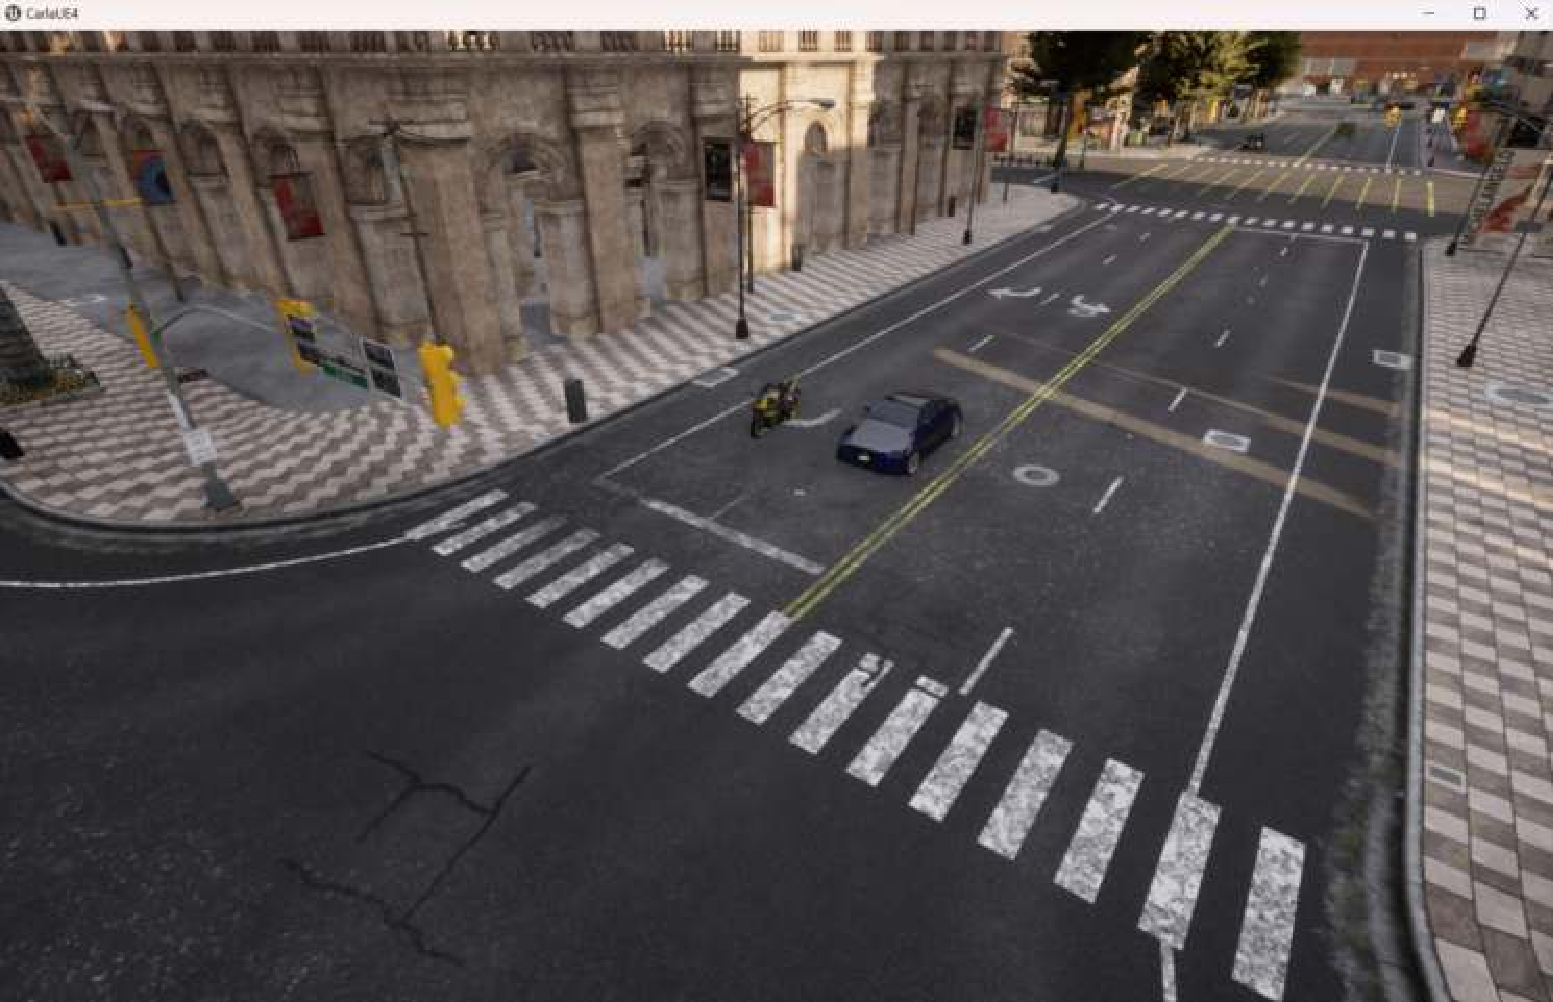
\includegraphics[width=0.8\textwidth]{"images/1.pdf"}
	\caption{摩托车与汽车在红绿灯前等待信号的场景截图}
	\label{fig:redlight_motorbike_car}
\end{figure}

\subsection{场景二:自我车辆在夜晚穿越道路}
\indent 在夜晚,一些自我车辆正在穿越道路,街道上的路灯微弱地照亮着周围环境,远处偶尔可以看到其他车辆的车灯闪烁。\\

\begin{figure}[H]
	\centering
	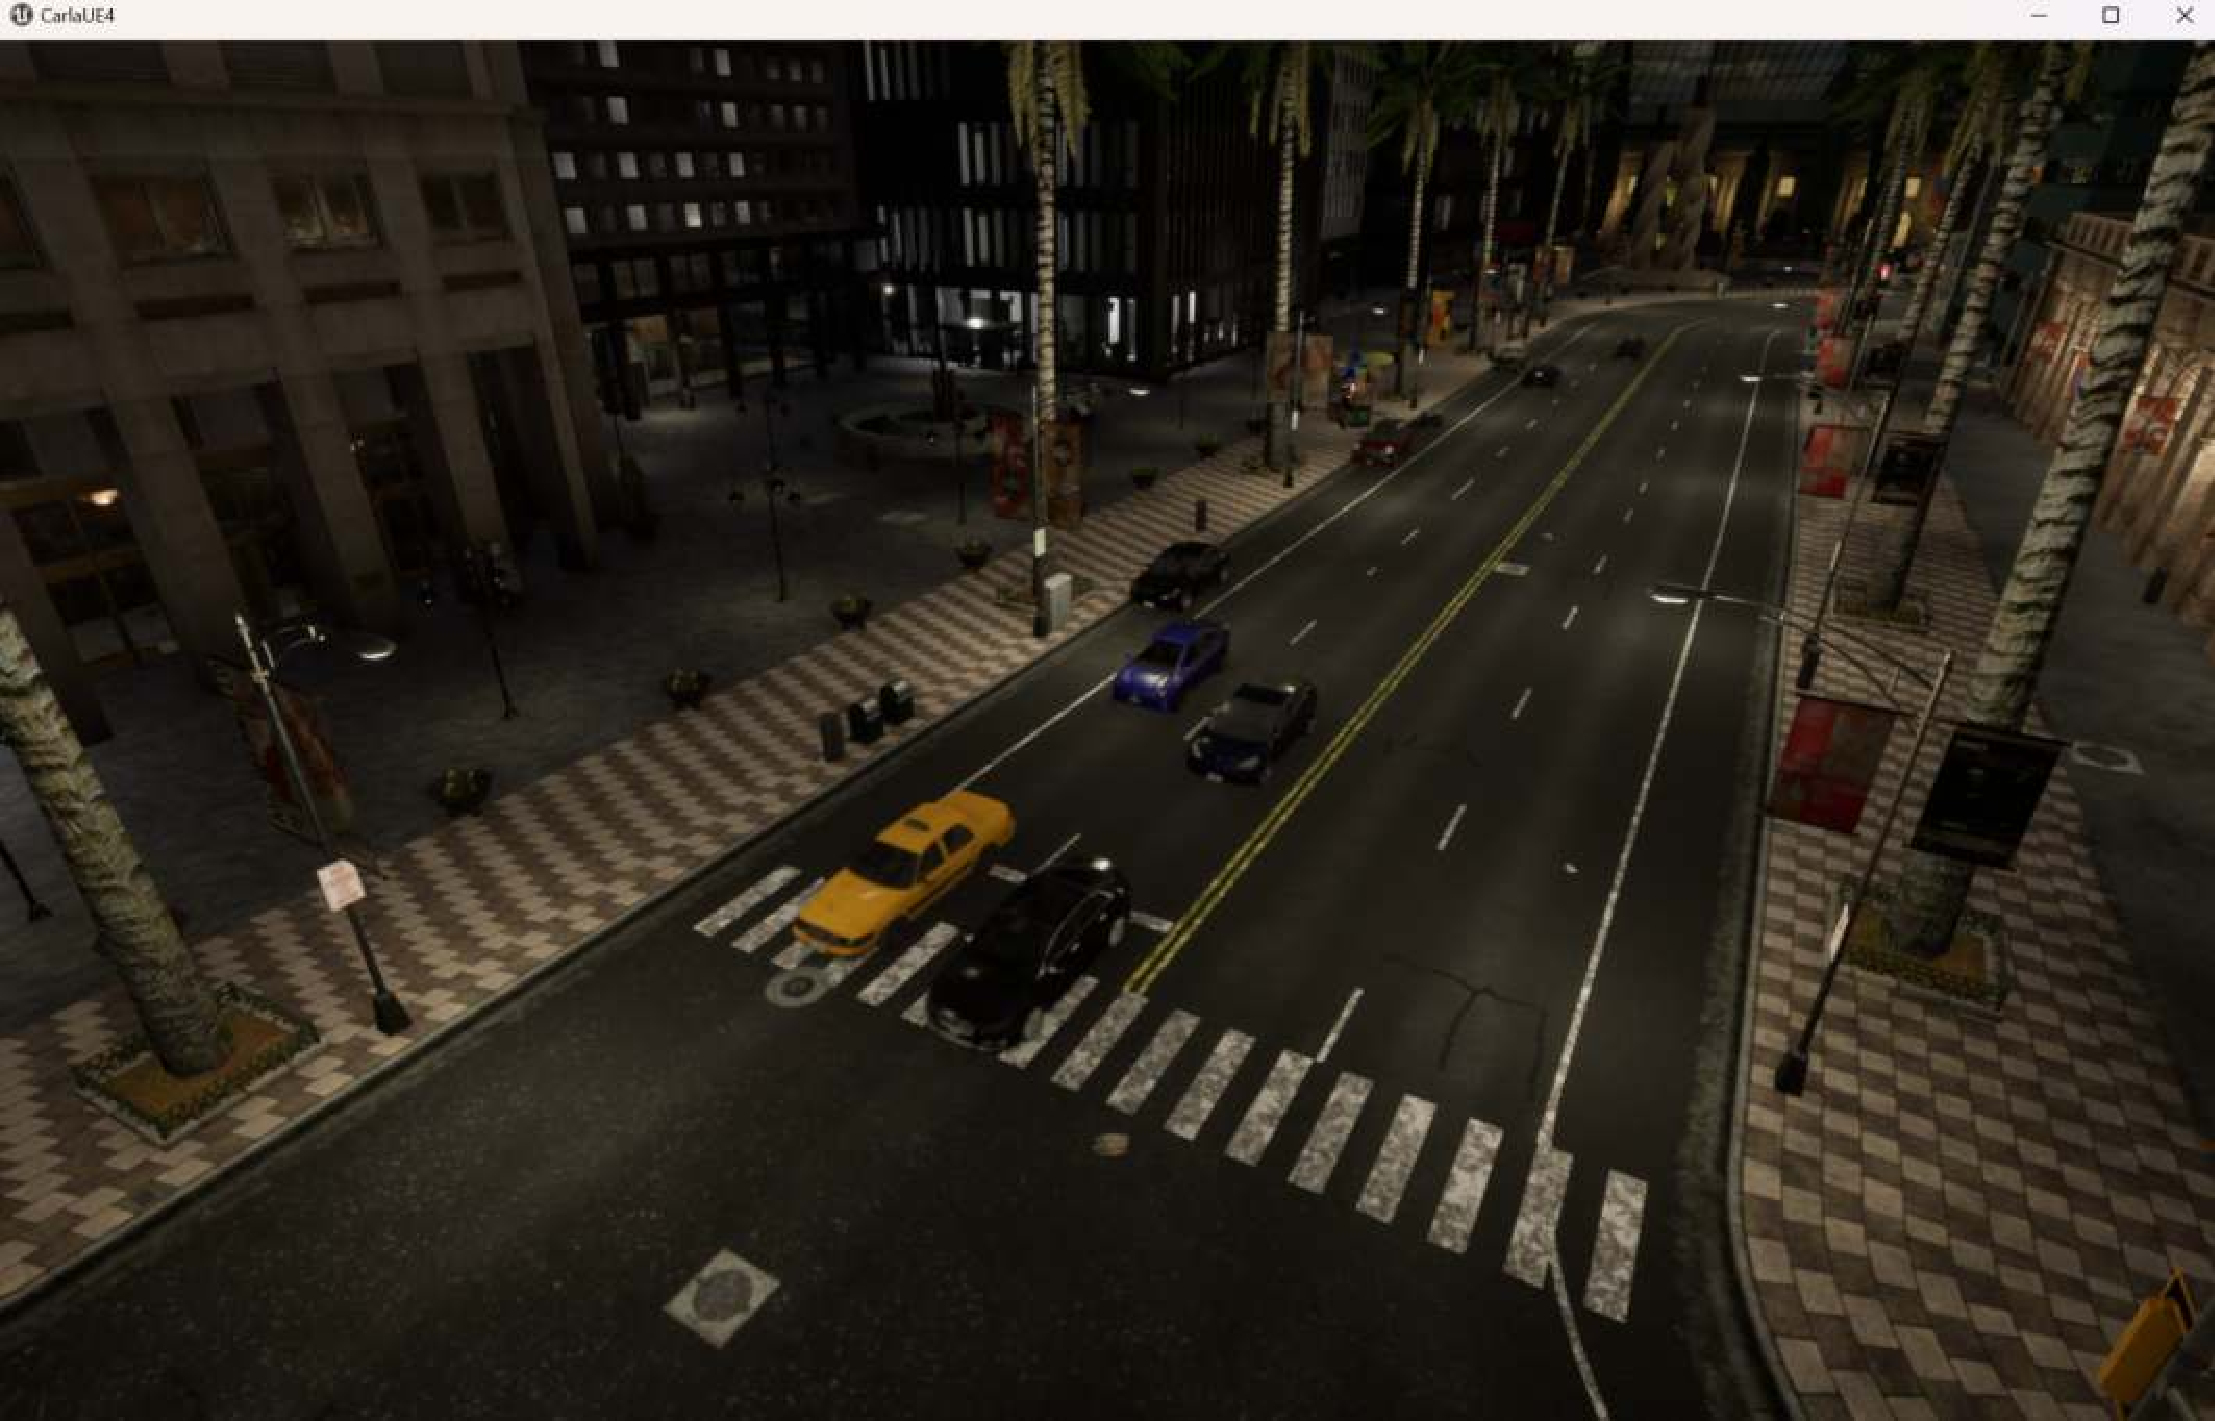
\includegraphics[width=0.8\textwidth]{"images/2.pdf"}
	\caption{自我车辆在夜晚穿越道路的场景截图}
	\label{fig:night_self_driving_cross}
\end{figure}

\subsection{场景三:自我车辆在夜晚红绿灯前等待信号}
\indent 在夜晚,一些自我车辆在红绿灯前等待信号,而在另一方向,自我车辆正在通行,车灯的光芒穿过昏暗的街道。\\

\begin{figure}[H]
	\centering
	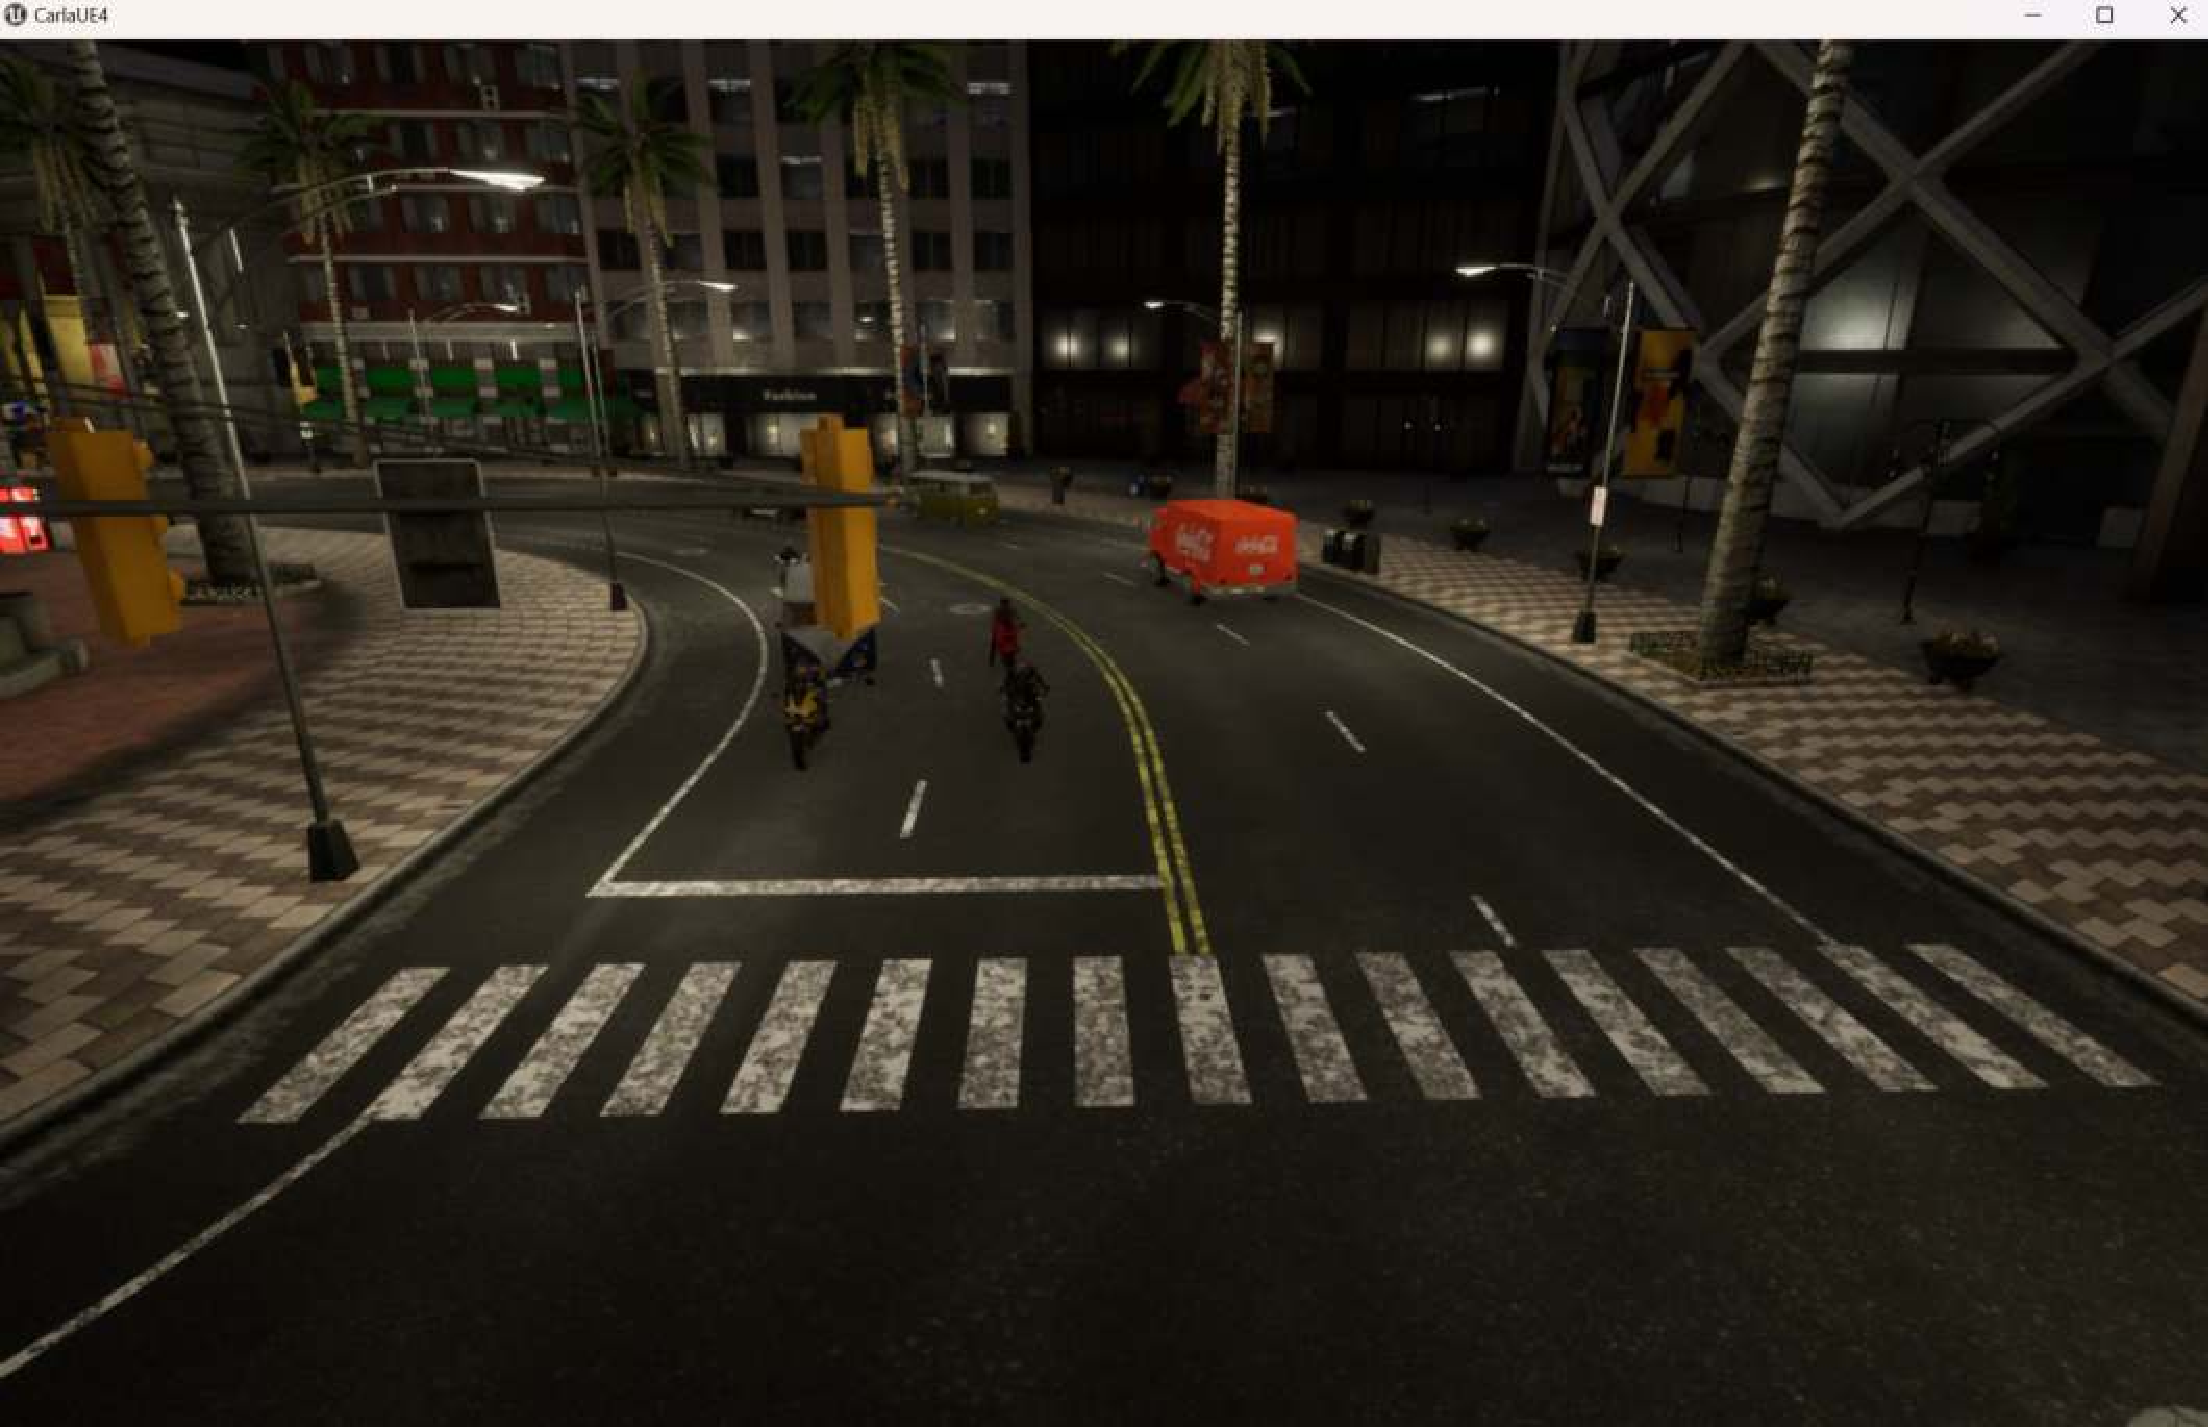
\includegraphics[width=0.8\textwidth]{"images/4.pdf"}
	\caption{自我车辆在夜晚红绿灯前等待信号的场景截图}
	\label{fig:night_redlight_cross}
\end{figure}

\subsection{场景四:行人横穿直行道路}
\indent 多辆自我车辆在笔直的道路上行驶时,一名行人突然从右前方横穿过来,并在自我车辆接近时突然停下。\\

\begin{figure}[H]
	\centering
	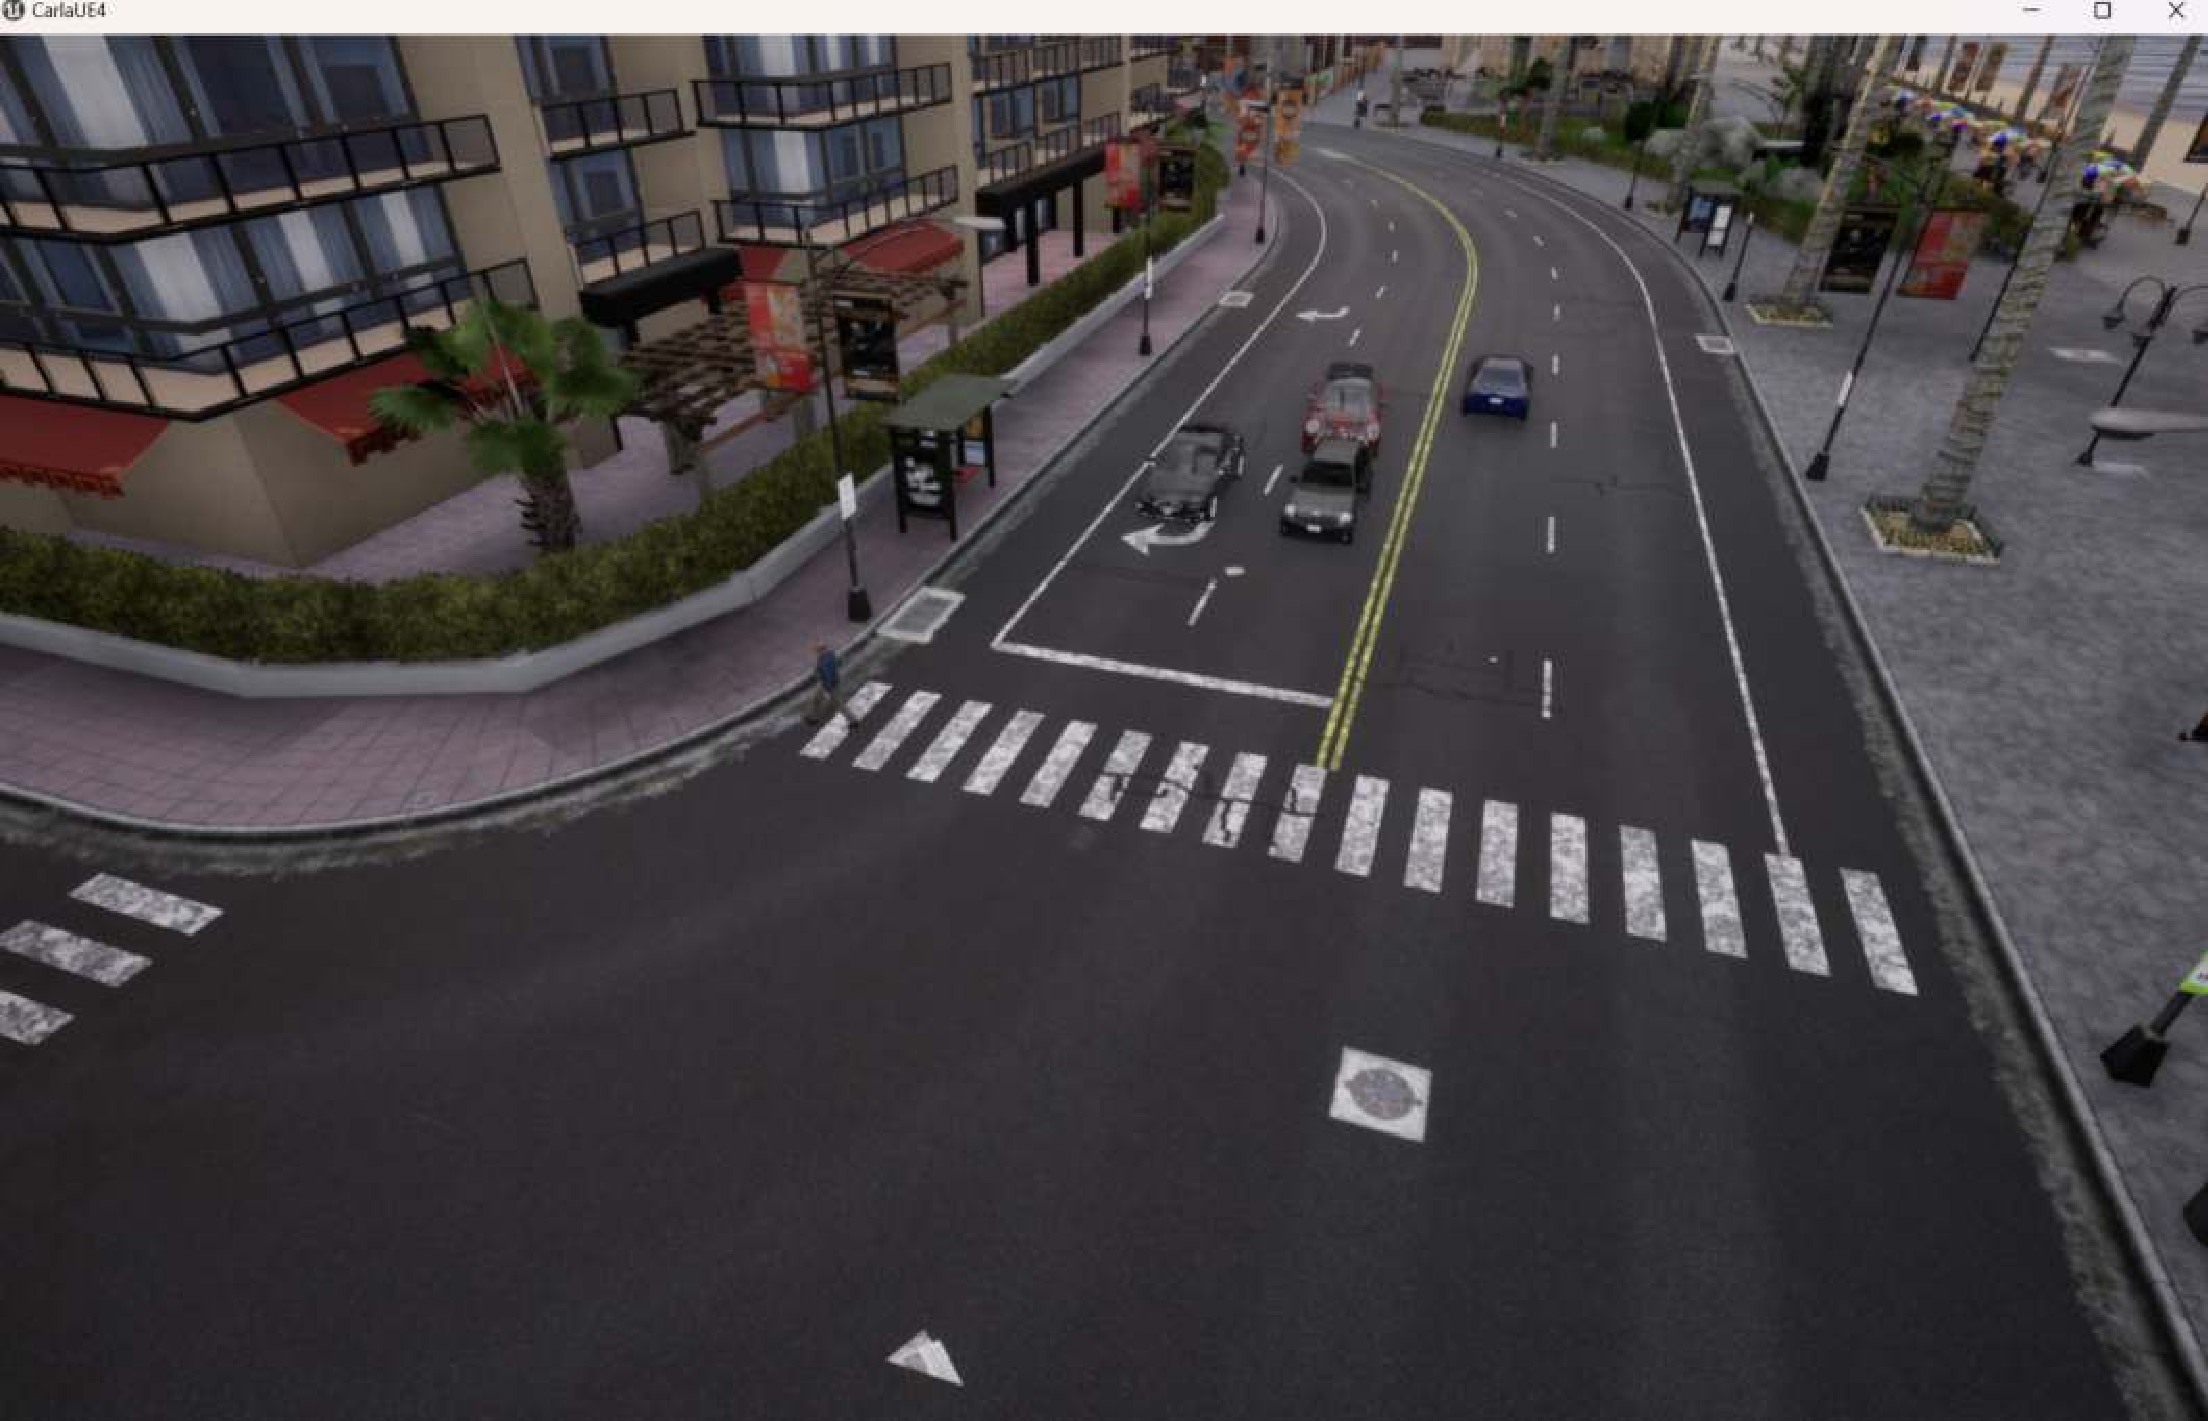
\includegraphics[width=0.8\textwidth]{"images/5.pdf"}
	\caption{行人横穿直行道路的场景截图}
	\label{fig:pedestrian_crossing}
\end{figure}
\subsection {场景五:自车在直路上行驶时,一名行人突然从右前方穿出}
\indent The ego vehicle is driving on a straight road when a pedestrian suddenly crosses from the right front and suddenly stops as the ego vehicle approaches.\\
\begin{figure}[H]
	\centering
	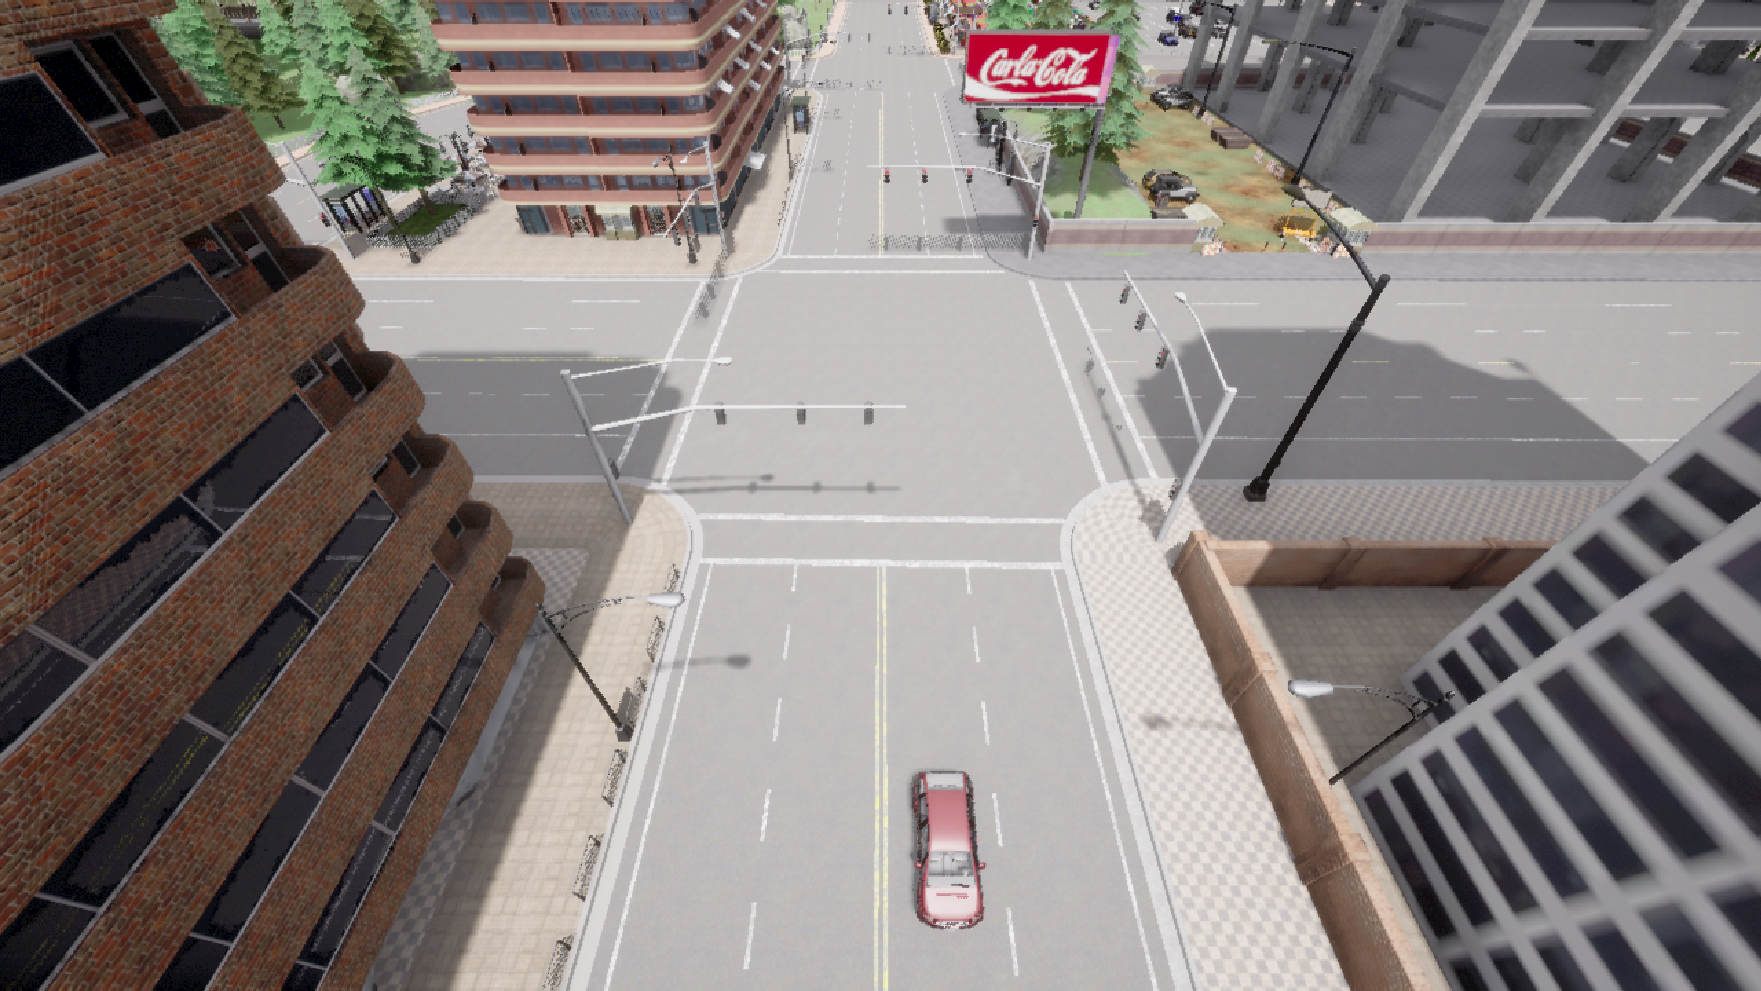
\includegraphics[width=0.8\textwidth]{"images/场景5.pdf"}
	\caption{场景截图}
	\label{}
\end{figure}
\subsection {场景六:自车在道路上行驶时,一名行人突然从左侧前方穿出}
\indent The ego vehicle is driving on a road when a pedestrian suddenly crosses from the left front and suddenly stops as the ego vehicle approaches.\\
\begin{figure}[H]
	\centering
	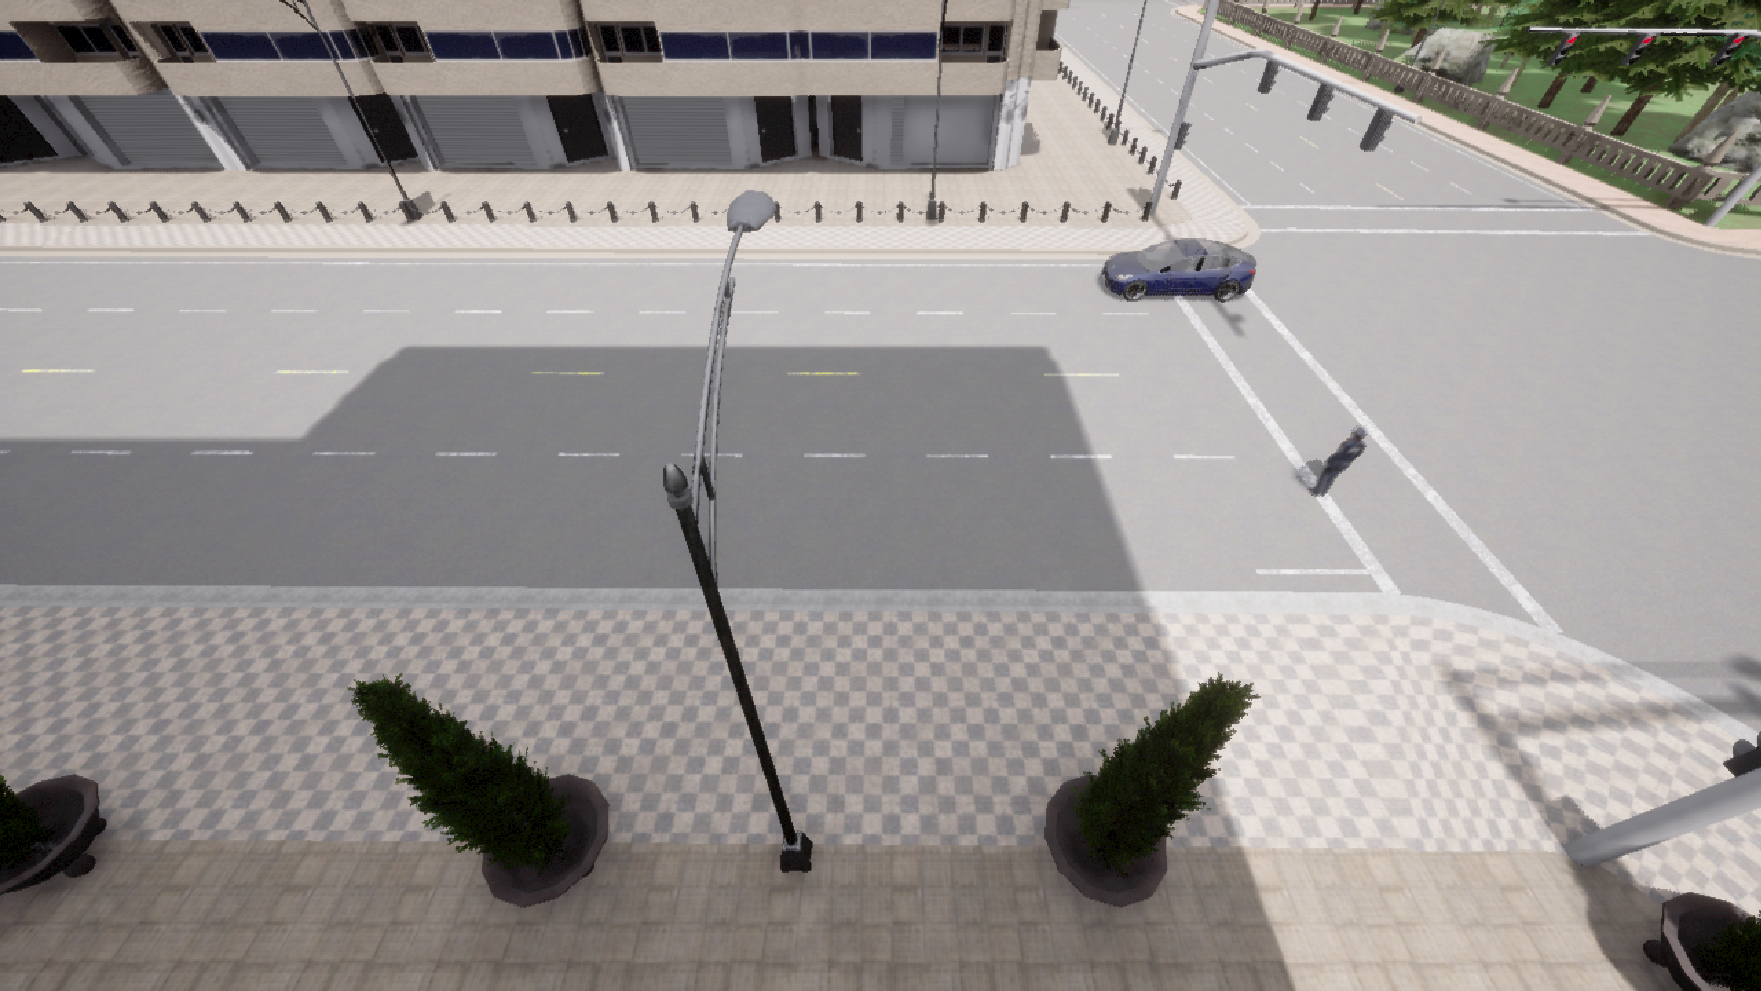
\includegraphics[width=0.8\textwidth]{"images/场景6.pdf"}
	\caption{}
	\label{}
\end{figure}
\subsection {场景七:两辆自车在直路上前后行驶}
\indent Two ego vehicles are driving in a straight line, one following the other.\\
\begin{figure}[H]
	\centering
	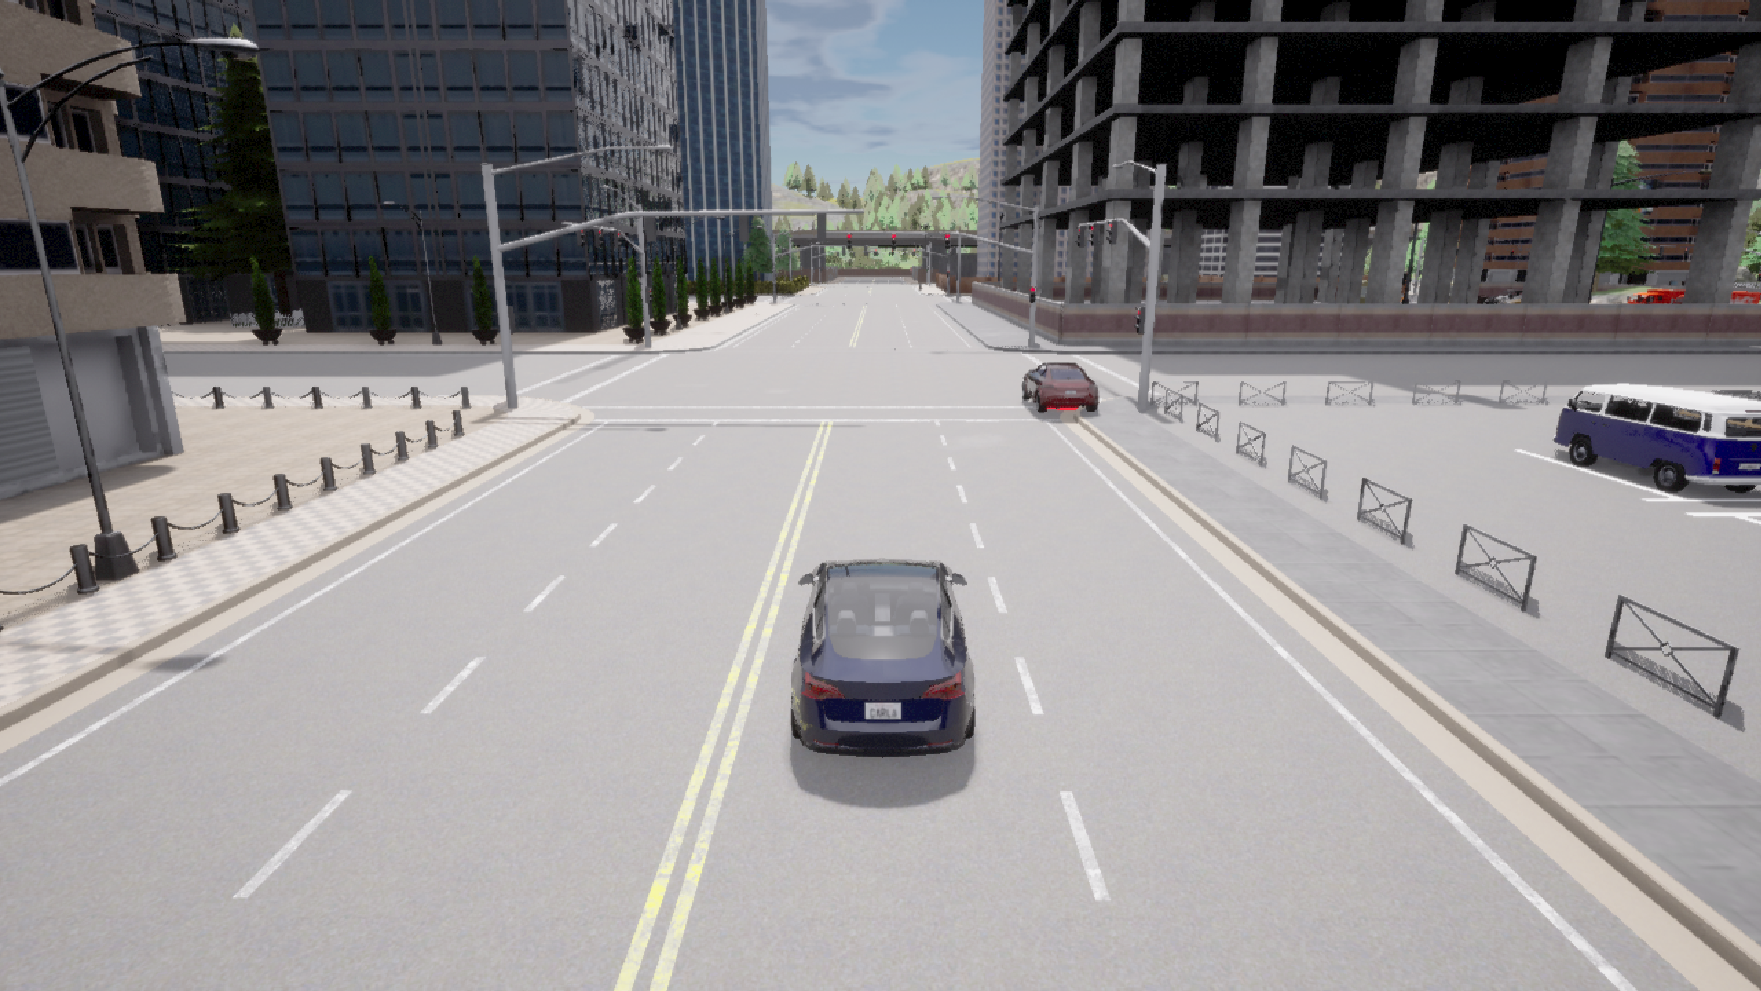
\includegraphics[width=0.8\textwidth]{"images/场景7.pdf"}
	\caption{}
	\label{}
\end{figure}
\subsection {场景八:一名行人横穿马路而自车在直到上行驶}
\begin{figure}[H]
	\indent A ego vehicle is driving on a straight road while a pedestrian is crossing the street.\\
	\centering
	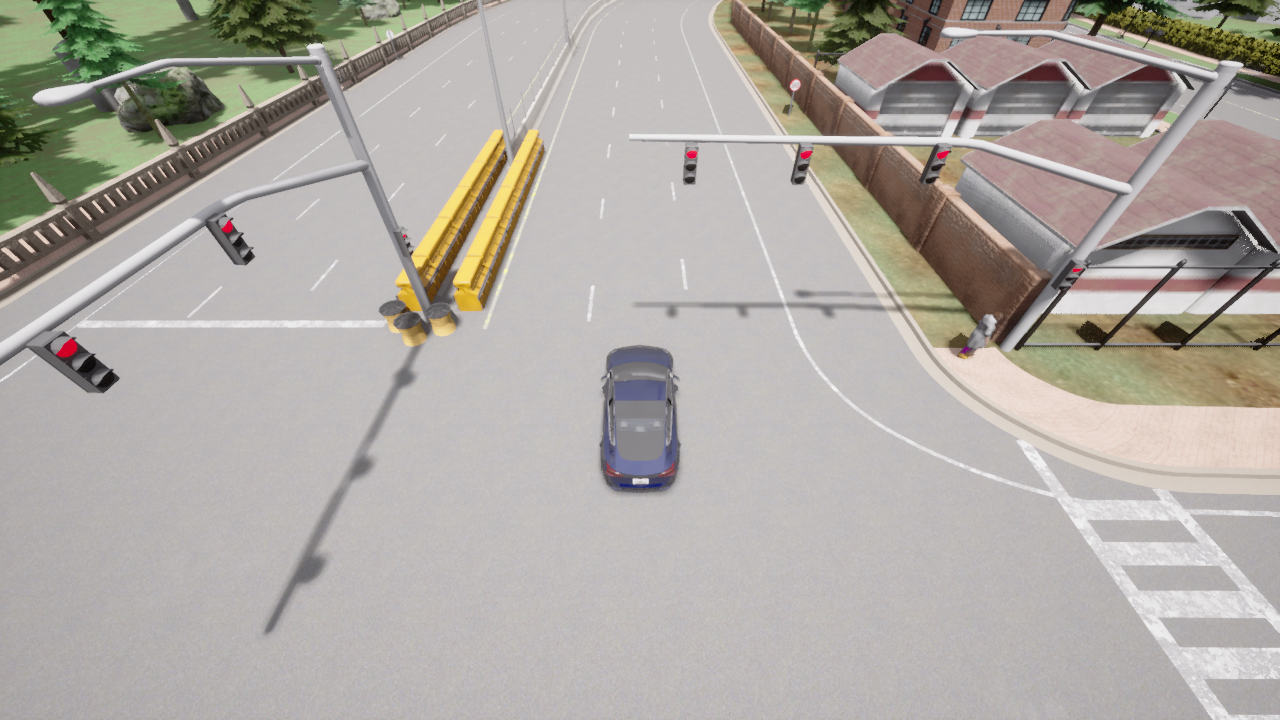
\includegraphics[width=0.8\textwidth]{"images/场景10.pdf"}
	\caption{}
	\label{}
\end{figure}
\subsection {场景九:夜晚行人在人行道上走}
\indent At night, a pedestrian is walking on the sidewalk.\\
\begin{figure}[H]
	\centering
	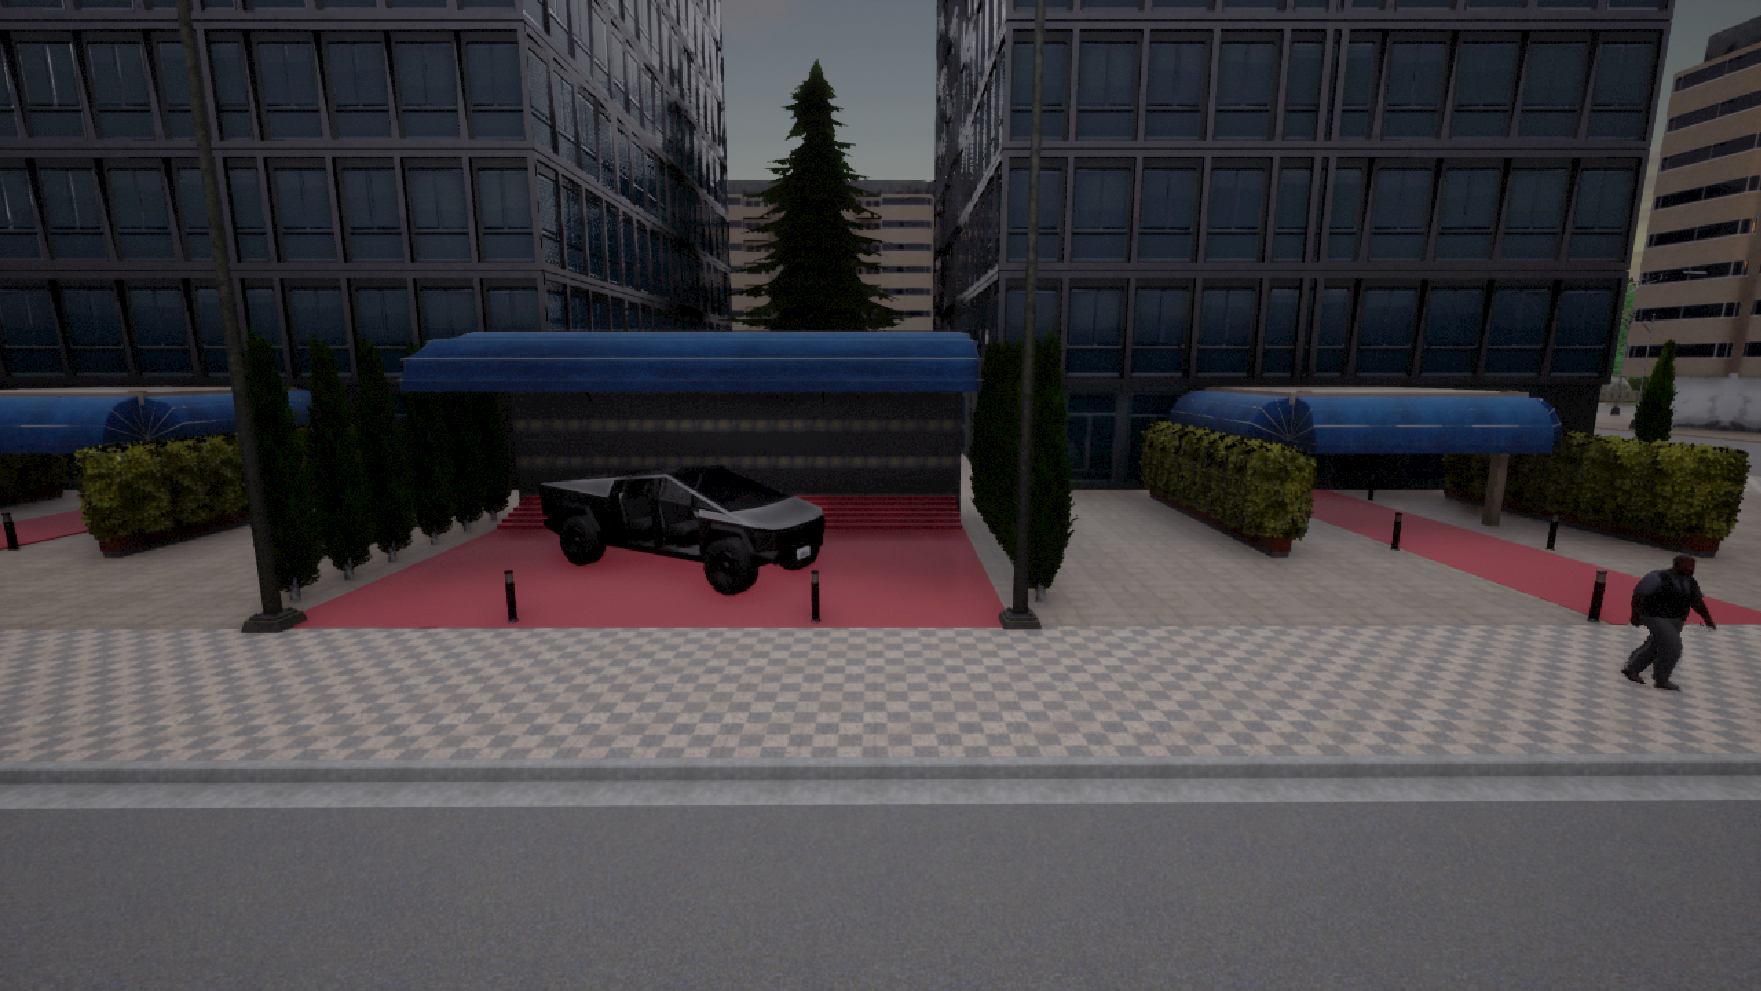
\includegraphics[width=0.8\textwidth]{"images/场景9.pdf"}
	\caption{}
	\label{}
\end{figure}
\subsection {场景十:自车通过十字路口}
\index The ego vehicle passes through the intersection.\\
\begin{figure}[H]
	\centering
	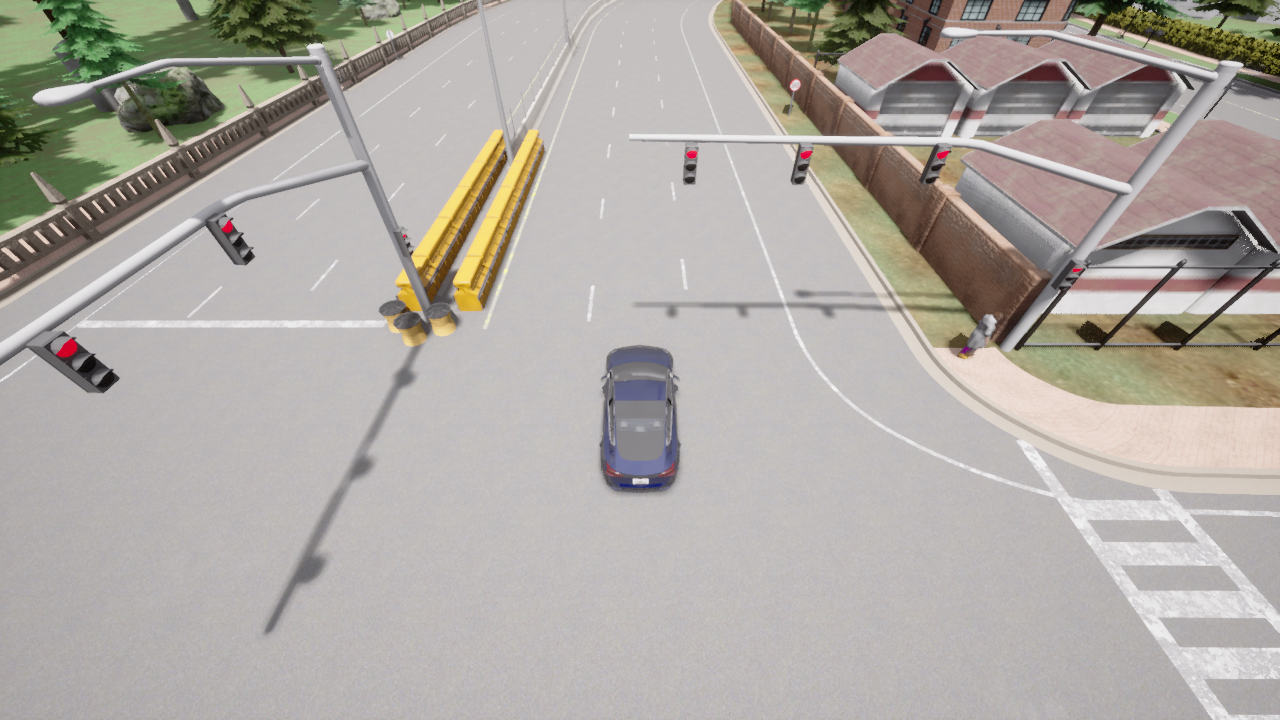
\includegraphics[width=0.8\textwidth]{"images/场景10.png"}
	\caption{}
	\label{}
\end{figure}


\section{评估测试分析}
为全面、客观地衡量本系统在从自然语言生成高保真三维交通场景过程中的表现,本文从语义保真度、场景多样性与系统效率三个核心维度构建了一套评估体系,具体指标设计如下:

(1)语义保真度(Semantic Fidelity):它主要是评估生成场景能不能准确还原输入自然语言里的核心语义信息,以此确保系统生成结果在语义层面有一致性和完整性。评估内容包含参与主体的一致性,像描述里提到的车辆类型比如红色轿车、卡车,还有行人、障碍物是否出现在仿真场景当中,空间位置关系,例如“在路口等待”“位于右侧车道”“靠近斑马线”等描述是否体现在实体布局里面,行为逻辑一致性,比如“等待绿灯”“直行通过”“与前车保持车距”等行为是否在仿真中能体现出来。评估方式采用检索式语义匹配评分也就是自动化加上人工评审打分也就是主观验证的双重手段,自动化方面是用自然语言处理模型计算输入描述和生成场景之间的语义相似度,主观方面是由3名评估者依据统一评分标准对每条样本进行1到5分打分,然后取平均作为最终得分。

(2)场景多样性(Scene Diversity):多样性评估用于衡量系统在面对不同自然语言输入时所生成场景之间的差异性,防止生成内容趋于模板化或重复模式。主要从以下几个角度度量:
1.结构多样性(Structure Diversity Score, SDS):通过提取场景中的车辆、行人、建筑等静态元素的布局特征,计算不同场景之间的结构差异程度;

2.行为多样性(Behavioral Diversity Score, BDS):通过仿真轨迹分析车辆在不同行为状态(加速、刹车、等待、避让等)上的变化情况,评估其动态多样性;

3.地图覆盖率方面要统计不同输入生成场景在CARLA地图里的分布情况,以此评估是否存在特定区域集中度过高的问题,采用像结构差异率、行为状态熵等定量指标来开展自动化评估工作,并且结合统计图表做可视化展示。

(3)系统效率与响应能力(Efficiency):系统效率是衡量该平台在真实应用场景下可行性的重要指标,重点考察系统从接收自然语言指令到输出完整三维场景所需的总时间开销,包括:检索耗时:Sentence-T5 向量化及相似描述查找所用时间;生成耗时:大语言模型生成 Scenic 脚本所耗时间;仿真加载与渲染时间:Scenic 编译后至 CARLA 仿真运行启动所经历的延迟;总响应时间:综合上述所有子流程,从输入自然语言到仿真画面出现的端到端时间。

通过日志记录还有脚本打点的方式来采集各个阶段的耗时,并且用平均响应时长(ms)、方差这类指标对性能表现进行量化,系统在多轮连续输入情况下的响应稳定性也被纳入评估范围。

在评估生成场景的质量时本研究选两种有代表性方法作基线对比,基于规则的方法即Rule - based这种方法通过定义明确逻辑和规则生成场景,它具有较好可解释性适合处理结构化和预定义任务,不过面对复杂和模糊的自然语言描述时灵活性和适应性较差,基于GPT - 4.0的方法借助大型语言模型生成能力来生成丰富多样的场景,该方法在场景生成多样性方面具备优势,不过在生成场景的物理合规性和逻辑一致性上存在不足,尤其是在处理复杂交通情境的时候。
选择这两种基线的主要目的是从不同角度评估本研究方法在生成场景质量、效率以及针对复杂和模糊指令的鲁棒性方面所具备的优势。\\
通过人工评估方式对 30 个生成场景进行语义一致性评分,得分范围为 0–5,得分越高表明语义表达越准确。结果如下\ref{tab:dependencies}:
\begin{table}[htbp]
	\centering
	\large % 放大字体
	\begin{tabular}{ll}
		\hline
		\textbf{评分区间} & \textbf{场景占比} \\
		\hline
		5分 & 0.62 \\
		4分 & 0.25 \\
		3分及一下 & 0.13 \\
		\hline
	\end{tabular}
	\caption{}
	\label{tab:dependencies}
\end{table}



平均得分为 4.38,说明生成系统在语义还原方面表现优异,能够较好地捕捉自然语言中的关键词及其空间/行为语义。

\subsection{准确率分析}
在输入条件近似的情况下,系统生成了具有多样参与者布局与动作的场景。采用结构特征编码后计算场景间欧几里得距离,多样性指标等,最后得出final Score平均约为 0.95,说明系统具备良好的准确率\ref{fig:accuracy_analysis}。
此外,通过对生成的截图进行视觉对比,发现系统在车辆类型、行驶方向、光照与天气等维度的变化也具备一定随机性与可控性。以下为两个评估测试的结果截图:
\begin{figure}[H]
	\centering
	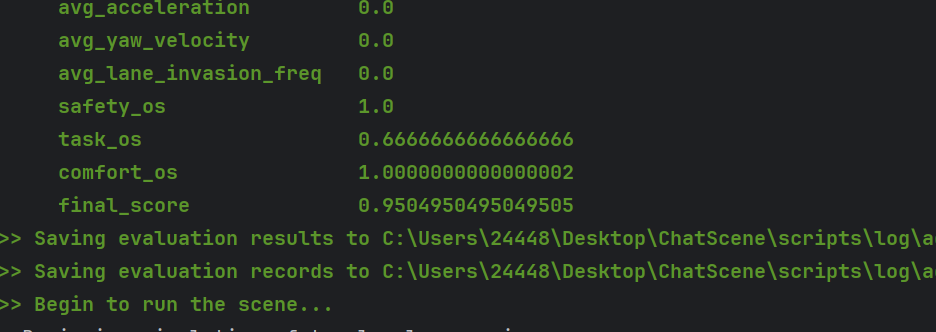
\includegraphics[width=0.8\textwidth]{"images/result2.pdf"}
	\caption{准确率分析1}
	\label{fig:accuracy_analysis}
\end{figure}

\begin{figure}[H]
	\centering
	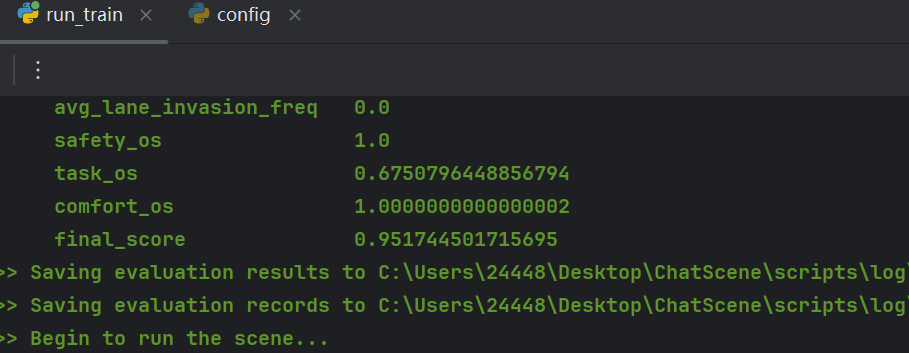
\includegraphics[width=0.8\textwidth]{"images/result1.pdf"}
	\caption{准确率分析2}
	\label{fig:accuracy_analysis}
\end{figure}

\subsection{效率分析}
系统整体生成流程的平均时间如下:
\begin{table}[H]
	\centering
	\begin{tabular}{ll}
		\hline
		\textbf{阶段} & \textbf{平均时间 (秒)} \\
		\hline
		语义检索与匹配 & 1.6 \\
		Scenic 脚本生成 & 2.3 \\
		Carla 场景加载与截图 & 4.3 \\
		\hline
		\textbf{总耗时} & \textbf{8.2} \\
		\hline
	\end{tabular}
	\caption{系统整体平均生成时间}
	\label{tab:system_generation_time}
\end{table}
为了验证系统在实际使用场景当中的运行效率,本文对从自然语言输入到三维仿真场景生成全过程的响应时间开展了测量与分析,系统整体生成流程的平均时间如下所示,通过上述统计能够看出,本系统在标准硬件配置的状况下可把一条自然语言指令完整转换为可视化交通场景的平均总耗时控制在9秒以内,具备较强的实时响应能力,在进行批量输入处理的时候,系统同样表现出良好的并发处理能力与稳定性。

经实验验证,在一次性处理20条自然语言输入的情形下,系统可在不显著增加响应时间的前提下完成全部场景的构建与仿真,平均每个场景的处理时间波动控制在±0.7秒范围内。
这表明:

(1)系统核心模块间的异步处理与缓存机制有效;

(2)大语言模型调用延迟已通过缓存和批处理策略优化;

(3) Scenic 与 CARLA 接口连接在高频调用场景下仍保持稳定。

总体来说系统拥有良好响应效率和可扩展性,不但支持单条交互式输入方式,而且能够满足批量生成相关需求,适合大规模自动驾驶测试等实际应用任务,比如仿真训练或者仿真场景库构建等,若要进一步提升系统的运行效率,可通过这些途径来进行优化:引入本地轻量化大模型以减少云端调用延迟;对检索模块进行并行化改造,提升向量查找速度;使用CARLA的异步仿真接口或地图预加载技术降低启动时间。
















